Data for this project was collected by the US. Army Corps of Engineers Engineer Research and Development Center (ERDC) in October 2015 at the Field Research Facility (FRF) in Duck, NC on the Outerbanks.\footnote{The data can be accessed online at http://chlthredds.erdc.dren.mil/thredds/catalog/frf/projects/bathyduck/catalog.html} The data was collected via the BathyDuck project conducted by the Coastal and Hydraulic Laboratory (CHL). Data of interest includes wave height, wave number, wave period, and bathymetry measurements. These data combine information collected by the Argus Beach Monitoring System, the Lighter Amphibious Resupply Cargo (LARC-5) vessel, and the Coastal Research Amphibious Buggy (CRAB). The latter two platforms are shown in Figure~\ref{crablarc}.

\begin{figure}[h]
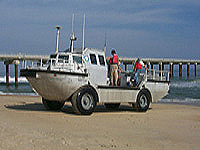
\includegraphics[width=.48\linewidth]{img/LARC.jpg}\hfill
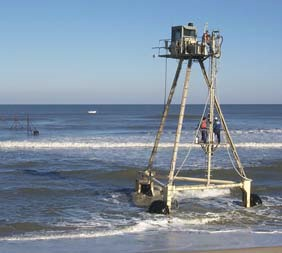
\includegraphics[width=.48\linewidth]{img/CRAB2.JPG}
\caption{The LARC (left) and CRAB (right) instruments are used to measure near coastal bathymetry. Image source: http://www.frf.usace.army.mil/aboutUS/equipment.shtml}
\label{crablarc}
\end{figure}

The following sections discuss in more detail the observations and how they were used. Please note that in physical space, the boundary point used for the 1D problem is located 1150 m offshore. For numerical simplicity all observations are transformed such that $\textit{x}$ = 0 m corresponds to the offshore boundary point and $\textit{x}$ = 1150 m is the shoreline. 

